These are basic models created using waijung library for a proper understanding of its simulink blocks.

\begin{figure}[hbt!]
    \centering
    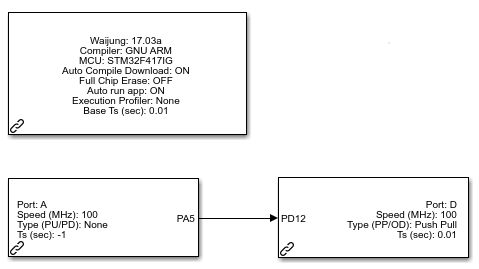
\includegraphics{digital input.png}
    \caption{Model for turning on LED by giving input to pin PA5}
\end{figure}

\begin{figure}[hbt!]
    \centering
    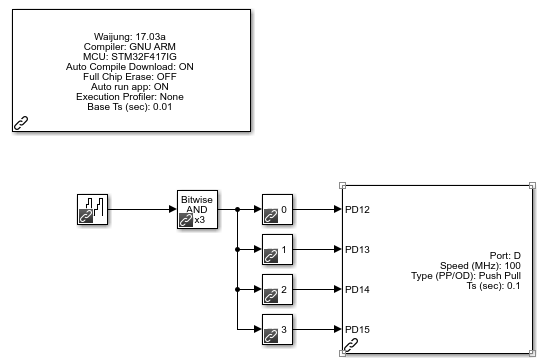
\includegraphics{digital output.png}
    \caption{Model for turning on/off led repeatedly.}
\end{figure}

\newpage
\begin{figure}[hbt!]
    \centering
    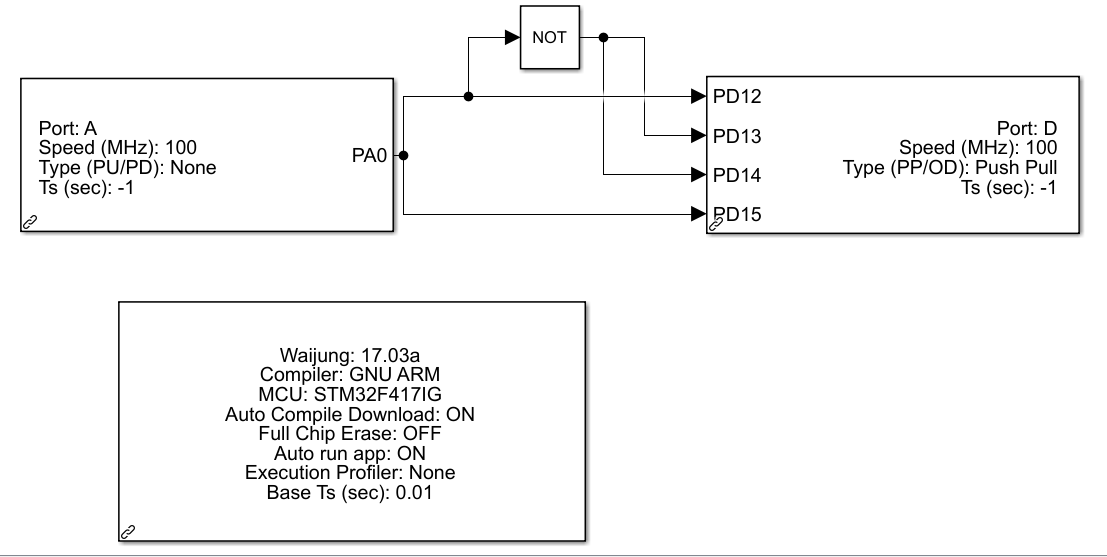
\includegraphics[width=14cm,height=9cm]{turiningonoffswitch.png}
    \caption{Model for switching on/off led by pressing switch.}
\end{figure}
